\Chapter{Implementáció}

Az implementációs fejezet részletesen bemutatja, hogyan valósultak meg a tervezési fázisban lefektetett elvek a konkrét kód szintjén. A fejezet a backend szolgáltatásoktól és adatmodellektől indul, majd a frontend állapotkezelésen és komponensstruktúrán át eljut a tesztelésig. Ahol indokolt, kódrészletek is szerepelnek az érintett mechanizmusok szemléltetéséhez.

% ─────────────────────────────────────────────────────────────────────────────
\Section{Backend implementáció}
% ─────────────────────────────────────────────────────────────────────────────

\SubSection{Projekt struktúra}

A backend kódja az alábbi könyvtárszerkezetbe szerveződik:

\begin{lstlisting}[language=bash, caption={Backend könyvtárstruktúra}]
backend/
  app.ts              # Express app konfiguráció, route regisztráció
  server.ts           # Szerver indítás, DB kapcsolat
  middleware/
    auth.ts           # JWT védő middleware
  models/             # Mongoose modellek (User, Project, Task, ...)
  routes/             # Express route handlerek
  controllers/        # Vezérlők (Task, GitHub)
  services/
    xpService.ts      # XP és szintlépési logika
    logService.ts     # Naplóbejegyzés írás
    githubService.ts  # GitHub API hívások
  config/
    db.ts             # MongoDB kapcsolat
  __tests__/          # Jest + Supertest integrációs tesztek
\end{lstlisting}

Az \texttt{app.ts} fájl az Express alkalmazást konfigurálja: engedélyezi a CORS-t, beállítja a JSON body parsert, és regisztrálja az összes route-ot a megfelelő előtag alá. Maga az Express app objektum exportálva van, és a \texttt{server.ts} indítja el a figyelő portot – ez a szétválasztás lehetővé teszi, hogy a tesztek közvetlenül az alkalmazáson fussanak anélkül, hogy valóban portot foglalnának.

\SubSection{Mongoose modellek}

A modellek TypeScript interfészeket definiálnak (\texttt{IUser}, \texttt{IProject} stb.), amelyek lehetővé teszik a típusbiztos hozzáférést a dokumentum mezőkhöz. Az alábbiakban a \texttt{User} modell megvalósításának főbb részei láthatók:

\begin{lstlisting}[language=JavaScript, caption={User modell (models/User.ts)}]
const UserSchema = new Schema<IUser>(
  {
    username: { type: String, required: true, unique: true },
    email:    { type: String, required: true, unique: true },
    password: { type: String, required: true },
    xp:       { type: Number, default: 0 },
    level:    { type: Number, default: 1 },
    prestige: { type: Number, default: 0 },
    role:     { type: String, default: 'user' },
  },
  { timestamps: true }
);
\end{lstlisting}

A \texttt{timestamps: true} beállítás automatikusan kezeli a \texttt{createdAt} és \texttt{updatedAt} mezőket. A \texttt{Project} modellben a kapcsolódó felhasználókat \texttt{Types.ObjectId} referenciákon keresztül tároljuk, amelyek a Mongoose \texttt{populate()} metódusával tölthetők ki tényleges adatokkal a lekérdezésekkor.

\SubSection{Hitelesítés implementációja}

A regisztrációs route (\texttt{POST /api/auth/register}) ellenőrzi az e-mail cím egyediségét, hasheli a jelszót, létrehozza a felhasználót, majd JWT tokent állít ki:

\begin{lstlisting}[language=JavaScript, caption={Regisztrációs végpont (routes/auth.ts)}]
router.post('/register', async (req, res) => {
  const { username, email, password } = req.body;
  const existingUser = await User.findOne({ email });
  if (existingUser)
    return res.status(400).json({ message: 'User already exists' });

  const hashedPassword = await bcrypt.hash(password, 10);
  const user = await User.create({ username, email,
                                   password: hashedPassword });

  const token = jwt.sign({ id: user._id },
    process.env.JWT_SECRET as string, { expiresIn: '7d' });

  res.status(201).json({ user, token });
});
\end{lstlisting}

A \texttt{protect} middleware dekódolja a Bearer tokent, megkeresi a felhasználót és csatolja a \texttt{req.user} mezőhöz. Ha a token érvénytelen vagy hiányzik, 401-es státuszkóddal tér vissza.

\SubSection{XP és gamifikációs szolgáltatás}

Az \texttt{xpService.ts} felelős az XP jóváírásáért és a szintlépési logikáért. A függvény egy \texttt{while} ciklusban ellenőrzi, hogy a felhasználó XP-je eléri-e a következő szinthez szükséges küszöbértéket, és ha igen, csökkenti az XP-t a küszöb értékével és növeli a szintet:

\begin{lstlisting}[language=JavaScript, caption={XP jóváírási logika (services/xpService.ts)}]
export const addXP = async (userId: string, xp: number) => {
  const user = await User.findById(userId);
  if (!user) throw new Error('User not found');
  user.xp += xp;

  const xpPerLevel = 100;
  while (user.xp >= user.level * xpPerLevel) {
    user.xp -= user.level * xpPerLevel;
    user.level += 1;
  }

  await user.save();
  return user;
};
\end{lstlisting}

Ez az implementáció kezeli azt az esetet is, amikor egyetlen feladat befejezésével a felhasználó egyszerre több szintet lép, mivel a \texttt{while} ciklus addig fut, amíg az XP az aktuális küszöb alatt nem kerül.

\SubSection{Naplózási szolgáltatás}

A \texttt{logService.ts} minden lényeges eseményt (feladat létrehozása, törlése, befejezése, sprint kezelés stb.) egy \texttt{Log} dokumentumként ment az adatbázisba. Fontos implementációs döntés, hogy a \texttt{logEvent} függvény hibáját soha nem engedi továbbugorni a hívó kódba: egy \texttt{try-catch} blokk belül a naplózási hiba csak konzolra kerül, így egyetlen rossz naplóbejegyzés sem törhet meg egy egyébként sikeres API hívást.

\SubSection{Projektlétrehozás TaskGroup-okkal}

A projektlétrehozási route megvalósítása összetett, mert egyszerre kell kezelni a projekt dokumentum létrehozását, a felhasználói referenciák feloldását felhasználóneveknél, és a taskGroup struktúrában érkező feladatok és alfeladatok tömegesen létrehozását. A route végigiterál a \texttt{taskGroups} tömbön, minden feladathoz létrehoz egy \texttt{Task} dokumentumot (a csoport határidejével), majd az alfeladatokhoz \texttt{Subtask} dokumentumokat kapcsol hozzá.

\begin{lstlisting}[language=JavaScript, caption={TaskGroup feldolgozás projektlétrehozáskor}]
for (const group of taskGroups) {
  if (!group.tasks) continue;
  for (const taskData of group.tasks) {
    const task = await Task.create({
      title: taskData.description,
      project: project._id,
      deadline: group.deadline,
    });
    if (taskData.subtasks) {
      for (const sub of taskData.subtasks) {
        await Subtask.create({ title: sub, task: task._id });
      }
    }
  }
}
\end{lstlisting}

% ─────────────────────────────────────────────────────────────────────────────
\Section{Webes frontend implementáció}
% ─────────────────────────────────────────────────────────────────────────────

\SubSection{Könyvtárstruktúra}

A webes frontend a következő főbb könyvtárakba szerveződik:

\begin{lstlisting}[language=bash, caption={Webes frontend könyvtárstruktúra}]
frontend/
  src/
    App.tsx               # Fő app, nézet routing
    main.tsx              # React DOM render, Providerek
    Context/
      GlobalContext.tsx   # Globális állapot Context
      ViewContext.tsx     # Nézet-váltás Context
      Reducer.tsx         # AppReducer (GlobalContext)
      ViewReducer.tsx     # ViewReducer
      Actions.ts          # Aszinkron action függvények
    components/
      Sidebar/            # Navigációs ikonok
      Topbar/             # Felső eszköztár komponensei
      Views/              # Nézetek (Kanban, Tasks, stb.)
      Sign/               # Bejelentkezés / regisztráció
      CreateProject/      # Projektlétrehozás varázsló
      Mails/              # Belső levelezés
      UserMenu/           # Profil oldal
    test/                 # Vitest + RTL unit tesztek
\end{lstlisting}

\SubSection{Context API és állapotkezelés}

A \texttt{GlobalContext} a \texttt{useReducer} hook segítségével kezel egy komplex állapotobjektumot. Az \texttt{AppReducer} minden lehetséges action típusra tartalmaz egy ágat, és mindig új állapotobjektumot ad vissza (immutable update). A \texttt{Actions.ts} fájl aszinkron action creator függvényeket tartalmaz, amelyek axios segítségével hívják az API-t, és dispatch hívásokkal frissítik a globális állapotot.

Az alábbi kódrészlet a feladatlekérési action megvalósítását mutatja be:

\begin{lstlisting}[language=JavaScript, caption={fetchTasks action (Context/Actions.ts)}]
export const fetchTasks = async (
  dispatch: Dispatch<any>,
  token: string,
  projectId: string,
) => {
  try {
    const res = await axios.get(
      `${API_URL}/tasks/project/${projectId}`,
      { headers: { Authorization: `Bearer ${token}` } },
    );
    dispatch({ type: 'SET_TASKS', payload: res.data });
  } catch (err: any) {
    dispatch({
      type: 'SET_ERROR',
      payload: err.response?.data?.message || err.message,
    });
  }
};
\end{lstlisting}

\SubSection{Nézetek implementációja}

Minden nézet-komponens (\texttt{TasksView}, \texttt{KanbanView}, \texttt{ScrumView} stb.) ugyanolyan struktúrát követ: a \texttt{useGlobalContext} hookkal hozzáfér az állapothoz, a \texttt{useEffect} hookkal a megfelelő adatokat tölti be (projekt-váltásra reagálva), és JSX-ben rendereli a tartalmat.

A \texttt{TasksView} komponens például az edíciós állapotot lokálisan, a \texttt{useState} hook segítségével kezeli: az \texttt{editingTask} állapot tartalmazza az éppen szerkesztett feladatot, és a kártya inline szerkesztési formát jelenít meg. A törlési és befejezési műveletek megfelelő API végpontokat hívnak, és a reducer az állapotot szinkron frissíti a szerver válasza alapján.

\begin{figure}[h!]
\centering
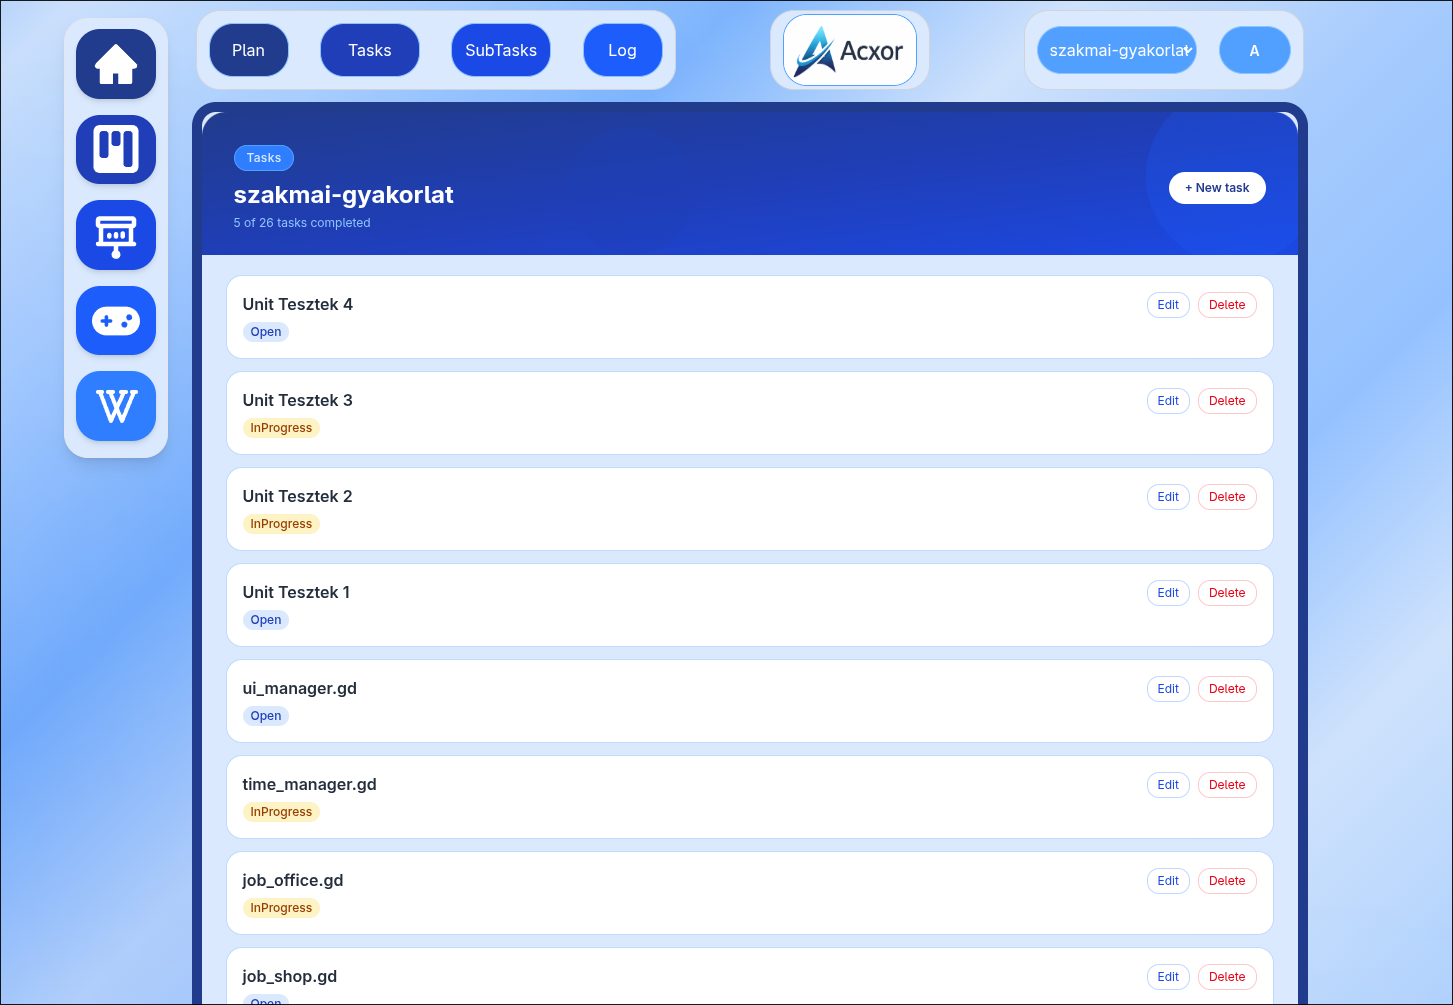
\includegraphics[width=0.8\textwidth]{images/frontend_tasks.png}
\caption{A TasksView komponens megjelenése}
\label{fig:architecture}
\end{figure}

\SubSection{Kanban nézet}

A \texttt{KanbanView} három oszlopban jeleníti meg a feladatokat (\texttt{Open}, \texttt{InProgress}, \texttt{Done}). Az oszlopok dinamikusan kiszámított adatokat kapnak: minden oszlop szűri a globális \texttt{tasks} tömbből a saját státuszához tartozó elemeket. Az oszlopok fejlécein megjelenik a benne lévő feladatok száma, az egyes kártyákon látható a felelős felhasználó és a határidő.

\begin{figure}[h!]
\centering
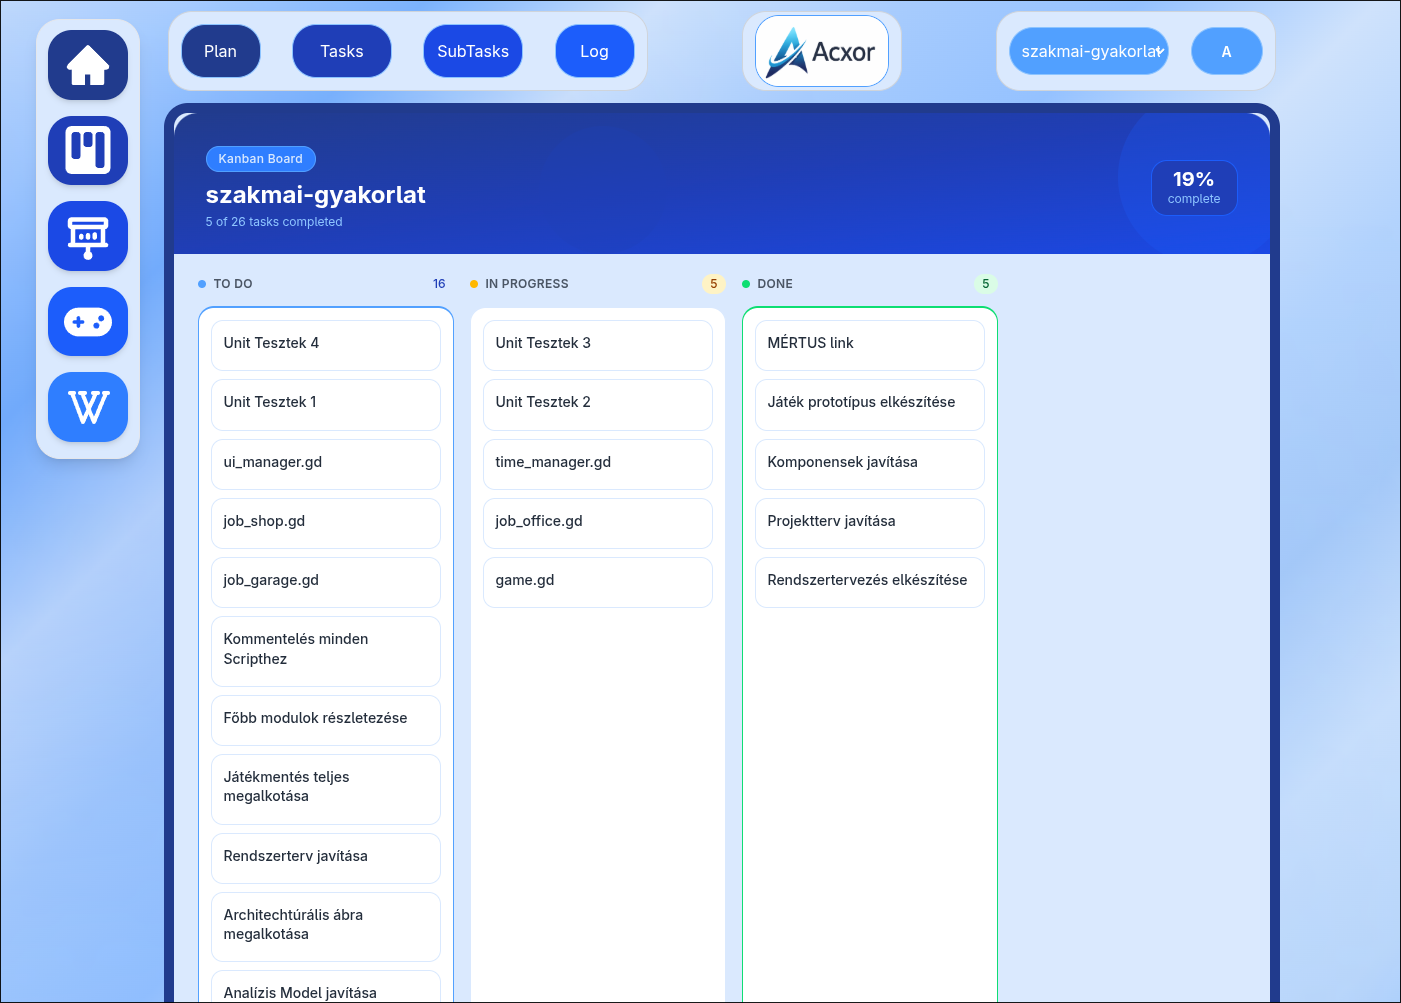
\includegraphics[width=0.8\textwidth]{images/frontend_kanban.png}
\caption{A KanbanView komponens megjelenése}
\label{fig:architecture}
\end{figure}

\SubSection{Scrum nézet}

A \texttt{ScrumView} a legösszetettebb nézetek egyike: egyszerre kezeli a sprint kiválasztást, sprint létrehozást, feladatok sprinthez rendelését, és a Kanban-szerű sprint boardot. A sprinthez nem rendelt feladatok a „Backlog" szekcióban jelennek meg. A sprint kiválasztó gombok tetején az aktív sprint (amelynek dátumtartománya lefedi az aktuális dátumot) egy zöld „active" badget kap. A sprint törlése után az érintett feladatok automatikusan visszakerülnek a backlogba (a backend kezeli ezt a konzisztenciát).

\begin{figure}[h!]
\centering
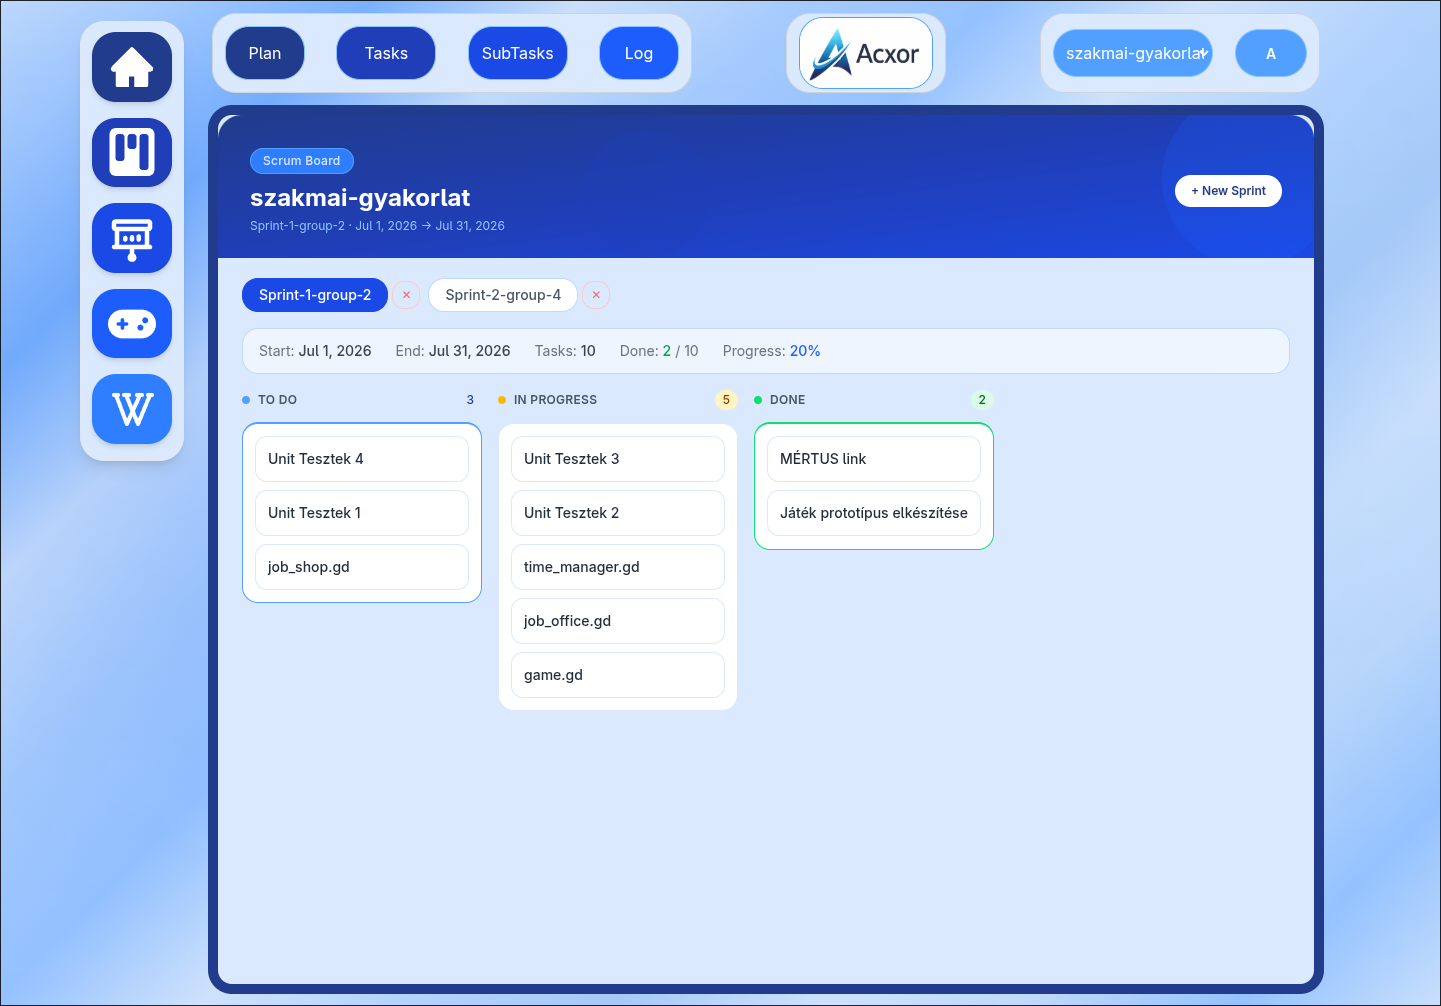
\includegraphics[width=0.8\textwidth]{images/frontend_scrum.png}
\caption{A ScrumView komponens megjelenése}
\label{fig:architecture}
\end{figure}

\SubSection{Gamifikáció nézet}

A \texttt{GamificationView} egy ranglistát jelenít meg a projekt tagjai számára. A felhasználókat XP és szint szerint rendezi, az első helyen lévő felhasználó kártyája arany szegéllyel kiemelve jelenik meg. Minden kártyán látható a felhasználó szintje, XP értéke, a következő szinthez szükséges XP, az XP progress bar és a megszerzett badge szintek. A gamifikációs rendszer magyarázatát egy kinyitható accordion panel tartalmazza, amelyben a szintlépési formula, a prestige rendszer és a class badge-ek kerülnek bemutatásra.

\begin{figure}[h!]
\centering
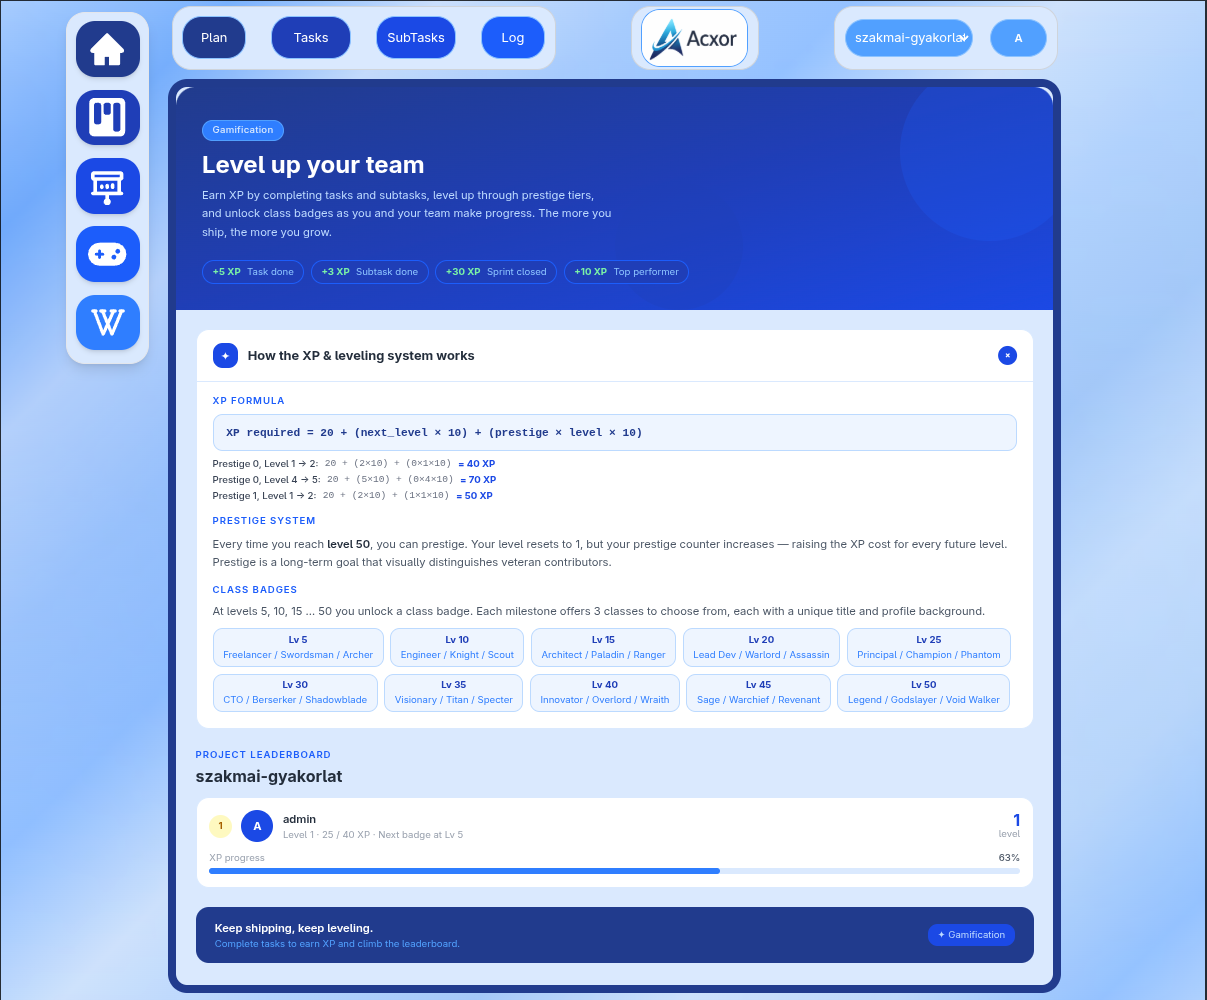
\includegraphics[width=0.8\textwidth]{images/frontend_game.png}
\caption{A GamificationView komponens megjelenése}
\label{fig:architecture}
\end{figure}

\SubSection{Mail rendszer}

A levelezési rendszer (\texttt{Mails} komponens) háromrészes elrendezést alkalmaz: egy hero fejléc, egy bal oldali levéllista panel (inbox / sent tab váltóval) és egy jobb oldali olvasó/szerkesztő panel. Az olvasási műveletnél a leveleket automatikusan olvasottnak jelöli a rendszer egy \texttt{PUT} kéréssel, és az olvasatlan levelek száma a hero fejlécben és az inbox tab feliratán is megjelenik. Az összeállítási nézet inline jelenik meg a jobb panelben, nem modálban.

% ─────────────────────────────────────────────────────────────────────────────
\Section{Mobil alkalmazás implementáció}
% ─────────────────────────────────────────────────────────────────────────────

\SubSection{Navigáció}

A mobil alkalmazás navigációja Expo Router segítségével valósul meg. A \texttt{(tabs)} csoportban tíz tab lap él: index (főoldal), tasks, subtasks, kanban, scrum, plan, gamification, mails, log, account. Az önálló képernyők (sign, create-project) a Stack navigátor részeként érhetők el. A tab bar egyedi komponensként lett megvalósítva (\texttt{CustomTabBar}), mivel az alapértelmezett Expo tab bar nem támogatta a vízszintes görgetést, amely tíz tab esetén szükségessé vált.

\begin{lstlisting}[language=JavaScript, caption={Egyedi tab bar implementáció (_layout.tsx)}]
function CustomTabBar({ state, navigation }) {
  return (
    <View style={styles.tabBarWrapper}>
      <ScrollView horizontal showsHorizontalScrollIndicator={false}>
        {TABS.map((tab, index) => {
          const focused = state.index === index;
          return (
            <TouchableOpacity
              key={tab.name}
              style={[styles.tabItem,
                      focused && styles.tabItemActive]}
              onPress={() => navigation.navigate(tab.name)}
            >
              {tab.icon(focused)}
              <Text style={[styles.tabLabel,
                            focused && styles.tabLabelActive]}>
                {tab.label}
              </Text>
            </TouchableOpacity>
          );
        })}
      </ScrollView>
    </View>
  );
}
\end{lstlisting}

\SubSection{Projekt választó}

Mivel a mobil alkalmazásban nincs topbar-szerű elem, a projektválasztás egy modal alapú \texttt{ProjectPicker} komponensen keresztül valósul meg. A komponens egy \texttt{TouchableOpacity} gombot jelenít meg az aktuális projekt nevével, és kattintásra egy alulról felcsúszó modal nyílik, amelyen az összes projekt listázva jelenik meg. A kiválasztott projekt azonnal frissíti a globális állapotot.

\SubSection{Alfeladatok nézet}

A mobil \texttt{SubtasksScreen} egy kinyitható/becsukható struktúrát alkalmaz: minden feladatkártya fejléce koppintható, és mutatja vagy elrejti az adott feladathoz tartozó alfeladatokat. Ez a döntés szükséges volt a mobilon elérhető kisebb képernyős terület miatt. Az alfeladatok hozzáadása inline szövegbeviteli mezőn keresztül, szerkesztésük pedig egy alulról felemelkedő modálban történik.

\SubSection{API kommunikáció}

A mobil alkalmazás a webes klienstől eltérően nem axio-st, hanem a beépített \texttt{fetch} API-t használja a HTTP kérésekhez. Ez tudatos döntés volt: csökkenti a függőségek számát, és a React Native fejlesztők által is preferált megoldás. Az API URL-t a \texttt{constants/api.ts} fájl konfigurálja dinamikusan: Expo Go fejlesztői módban a \texttt{Constants.expoConfig.hostUri} alapján automatikusan meghatározza a fejlesztői gép LAN IP-jét, így fizikai eszközön is működik a fejlesztés.

\begin{lstlisting}[language=JavaScript, caption={Dinamikus API URL (constants/api.ts)}]
const debuggerHost =
  Constants.expoConfig?.hostUri?.split(':')[0];

const BASE = debuggerHost
  ? `http://${debuggerHost}:5000/api`
  : 'http://localhost:5000/api';

export const API_URL = BASE;
\end{lstlisting}

\begin{figure}[h!]
\centering
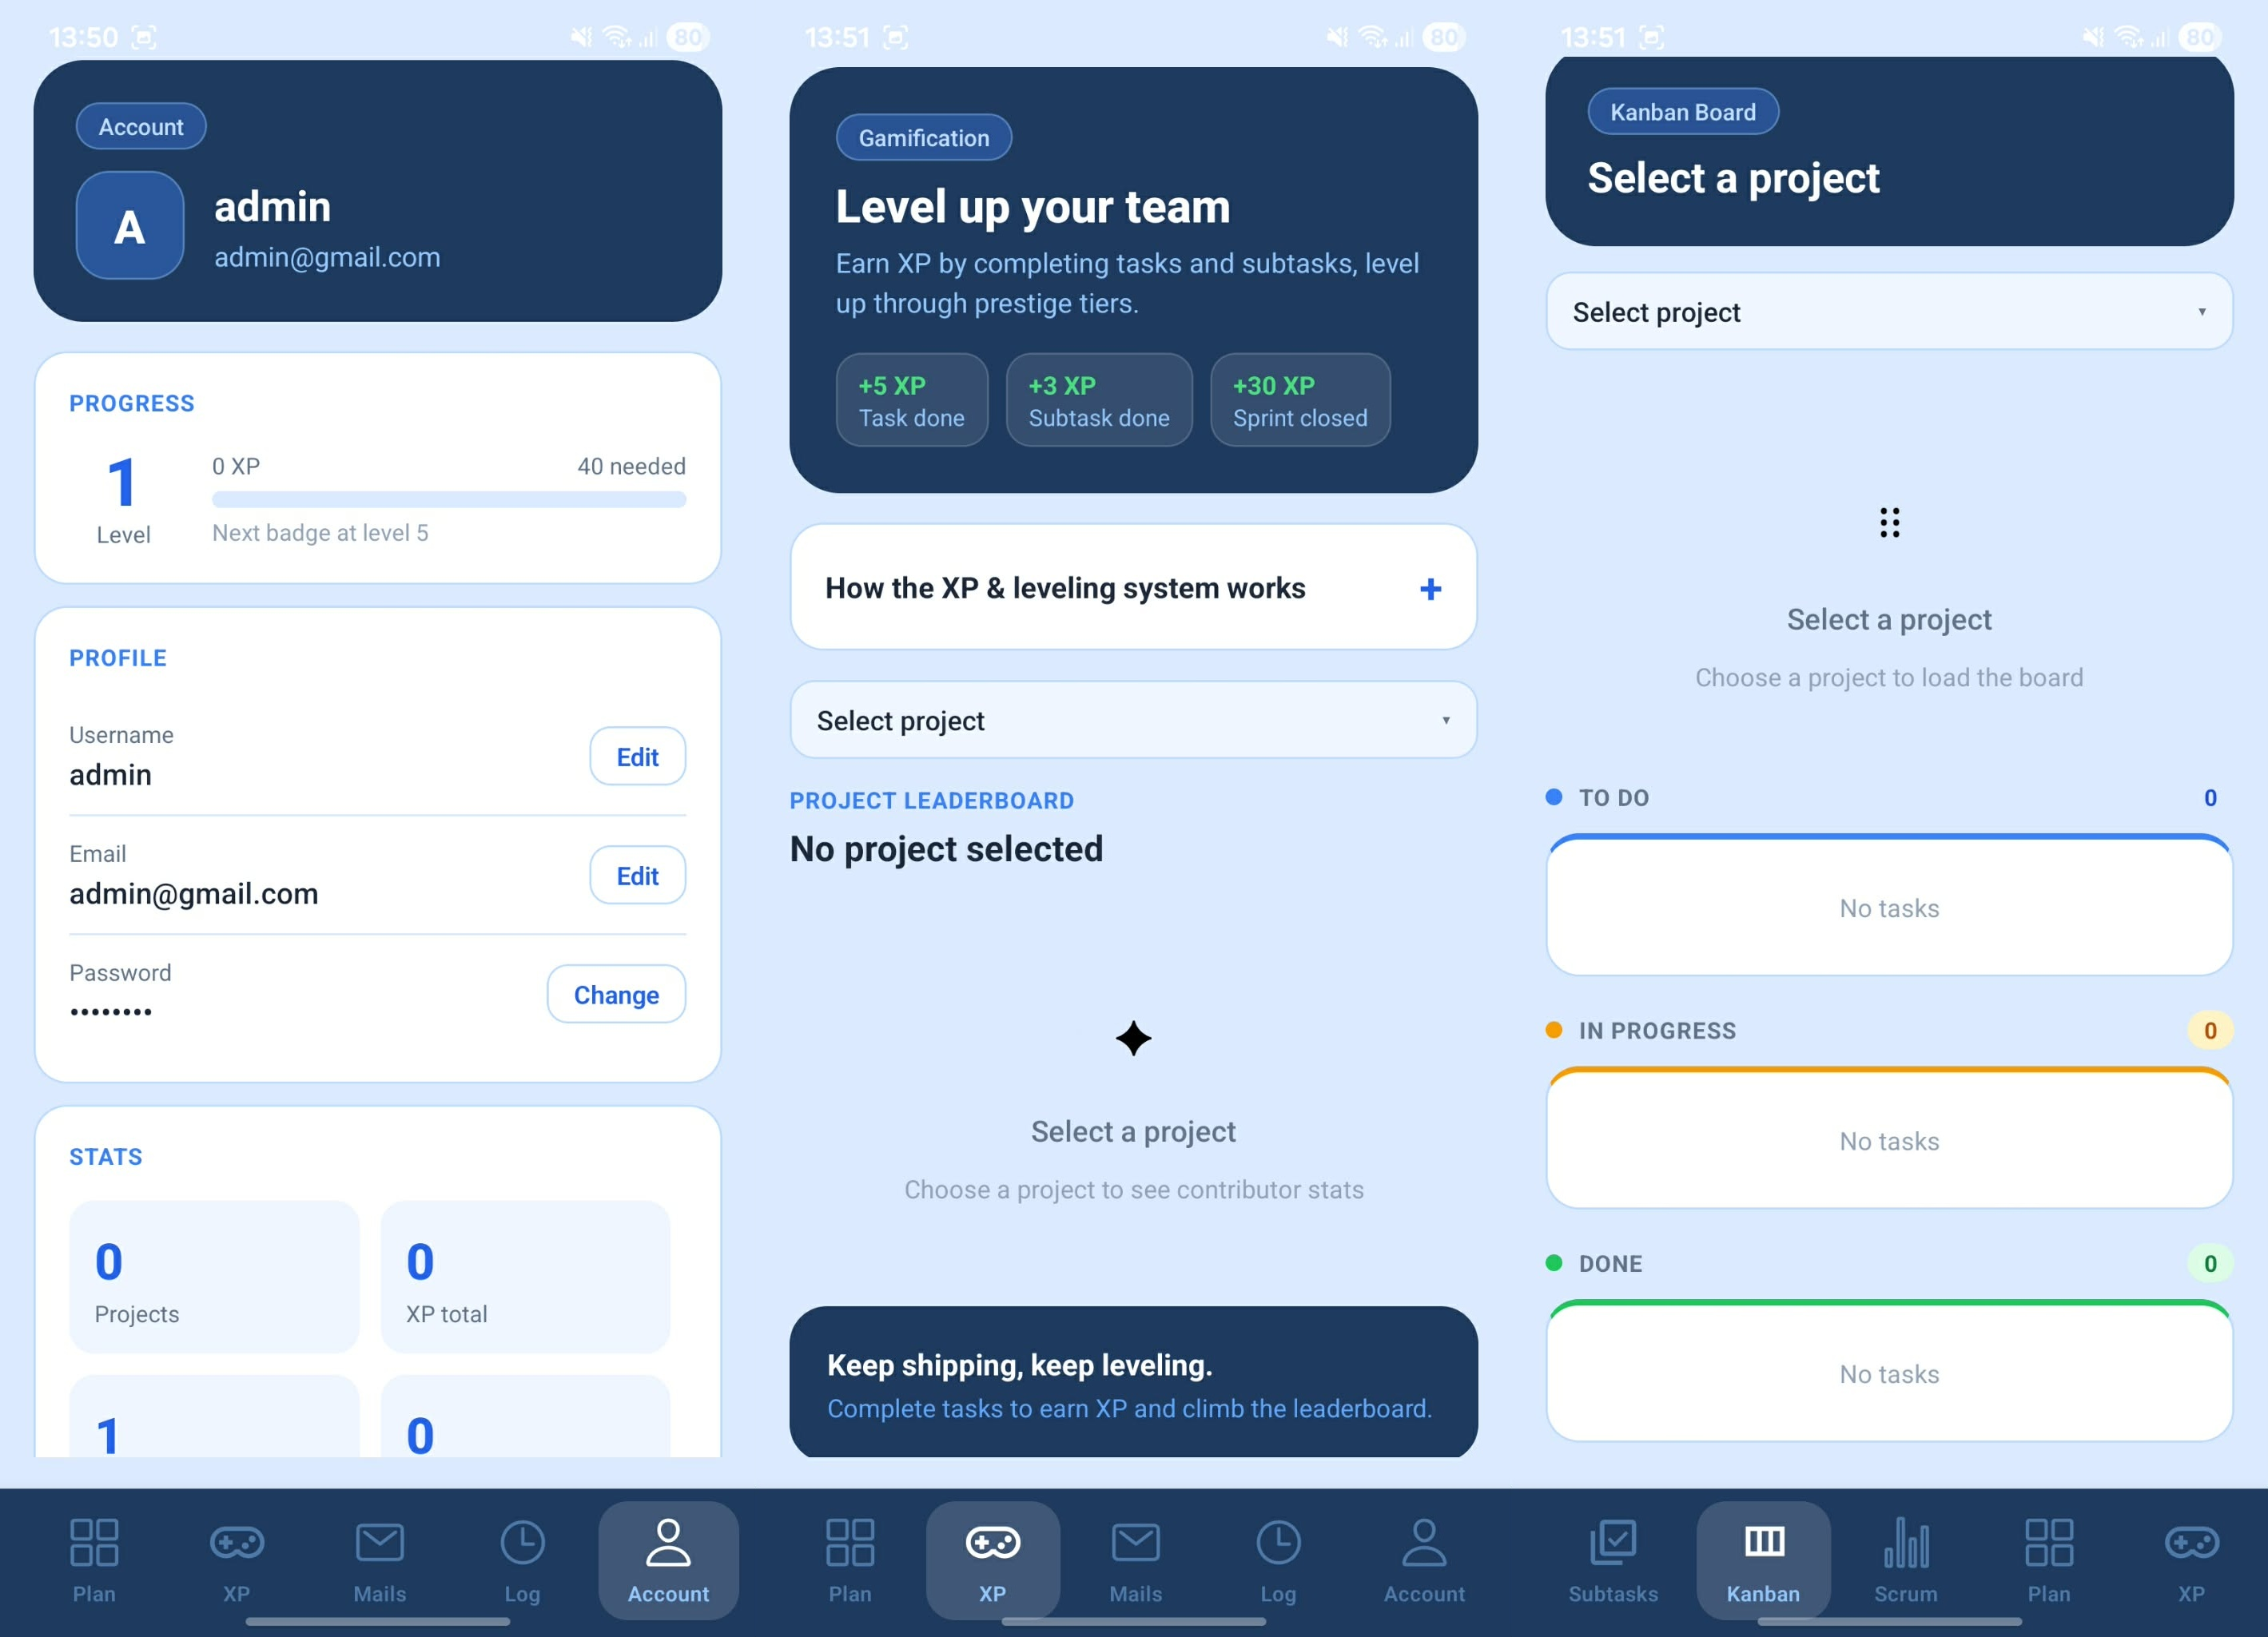
\includegraphics[width=0.8\textwidth]{images/mobile_screens.png}
\caption{A mobil alkalmazás főbb nézetei}
\label{fig:architecture}
\end{figure}

% ─────────────────────────────────────────────────────────────────────────────
\Section{Tesztelés implementációja}
% ─────────────────────────────────────────────────────────────────────────────

A rendszer tesztelése két szinten valósul meg: backend oldalon Jest és Supertest segítségével írt integrációs tesztek, frontend oldalon Vitest és React Testing Library alapú unit tesztek.

\SubSection{Backend tesztelés}

A backend tesztek in-memory MongoDB adatbázist alkalmaznak (\texttt{mongodb-memory-server}), ami azt jelenti, hogy a tesztek nem igényelnek élő adatbázis-kapcsolatot, és teljesen izoláltan futnak. A \texttt{setup.ts} fájl minden tesztfájl előtt elindítja a memóriaadatbázist, és minden egyes teszt után törli az összes kollekcióból az adatokat, hogy biztosítsa az izolált futtatást.

\begin{lstlisting}[language=JavaScript, caption={Teszt setup (\_\_tests\_\_/setup.ts)}]
beforeAll(async () => {
  mongoServer = await MongoMemoryServer.create();
  await mongoose.connect(mongoServer.getUri());
});

afterEach(async () => {
  const collections = mongoose.connection.collections;
  for (const key in collections)
    await collections[key].deleteMany({});
});

afterAll(async () => {
  await mongoose.disconnect();
  await mongoServer.stop();
});
\end{lstlisting}

Az integrációs tesztek a Supertest könyvtár segítségével közvetlenül az Express alkalmazásnak küldenek HTTP kéréseket, és ellenőrzik a visszakapott státuszkódot, a válasz testét és az adatbázis állapotát. A tesztek lefedik az auth, project, task, subtask és service szintű működést.

\begin{figure}[h!]
\centering
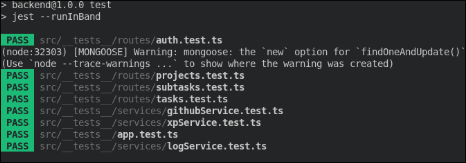
\includegraphics[width=0.8\textwidth]{images/jest_tests.png}
\caption{A backend tesztek futtatásának eredménye}
\label{fig:architecture}
\end{figure}

\SubSection{Frontend tesztelés}

A webes frontend tesztjei Vitest és React Testing Library segítségével készültek. A tesztek négy fő területet fednek le:

\begin{enumerate}
\item \textbf{Reducer tesztek}: Az \texttt{AppReducer} és \texttt{ViewReducer} függvények elszigetelt tesztelése, verifikálva, hogy minden action típus a várt állapotváltozást eredményezi.
\item \textbf{Context tesztek}: A \texttt{GlobalContext} és \texttt{ViewContext} tesztelése egyszerű tesztkomponenseken keresztül, ellenőrizve a dispatch-re adott re-render viselkedést.
\item \textbf{Action tesztek}: A \texttt{fetchTasks} és \texttt{addTask} action creator függvények tesztelése mockolt axios segítségével, verifikálva a helyes API hívást és dispatch sorozatot.
\item \textbf{Komponens tesztek}: A \texttt{Sign}, \texttt{CreateProject}, \texttt{TasksView} és \texttt{SubTasksView} komponensek renderelési és interakciós tesztjei, mockolt Context segítségével.
\end{enumerate}

\begin{lstlisting}[language=JavaScript, caption={TasksView unit teszt (Vitest)}]
it('rendereli a TasksView-t', () => {
  vi.spyOn(GlobalContext, 'useGlobalContext').mockReturnValue({
    state: {
      tasks: [
        { _id: '1', title: 'Task 1', status: 'open' },
        { _id: '2', title: 'Task 2', status: 'done' },
      ],
      selectedProject: { _id: 'proj1' },
      // ... egyéb mezők
    },
    dispatch: vi.fn(),
  });

  render(<TasksView />);
  expect(screen.getByText('Tasks')).toBeInTheDocument();
  expect(screen.getByText('Task 1')).toBeInTheDocument();
  expect(screen.getByText('Task 2')).toBeInTheDocument();
});
\end{lstlisting}

\begin{figure}[h!]
\centering
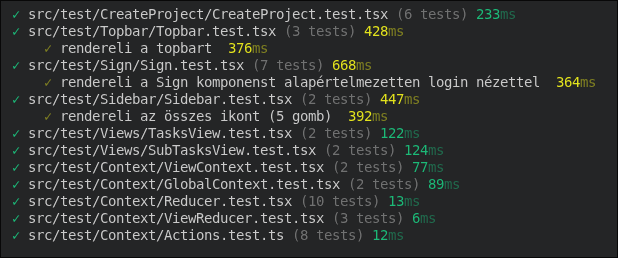
\includegraphics[width=0.8\textwidth]{images/vitest_tests.png}
\caption{A frontend tesztek futtatásának eredménye}
\label{fig:architecture}
\end{figure}

\SubSection{GitHub service tesztelés}

A \texttt{githubService.ts} tesztelése érdekes kihívást jelentett, mivel a GitHub API-t nem szerettük volna valóban hívni a tesztek során. Az axios mockolt verziójával (\texttt{jest.mock('axios')}) a tesztek ellenőrzik, hogy a service függvények a helyes URL-t hívják-e, a helyes headereket küldik-e el, és a válasz adatait a várt formátumra alakítják-e. A \texttt{logService.ts} tesztelésénél a \texttt{console.log} spy-olásával ellenőriztük, hogy a naplóbejegyzések a várt formátumban kerülnek kiírásra.

% ─────────────────────────────────────────────────────────────────────────────
\Section{Fejlesztési kihívások és megoldások}
% ─────────────────────────────────────────────────────────────────────────────

A fejlesztés során számos praktikus kihívással kellett szembenézni, amelyek megoldása tanulságos volt.

\textbf{Alfeladat betöltés párhuzamos kérésekkel}: Az alfeladatokat feladatonként kellett betölteni, ami azt jelentette, hogy ha egy projektnek 10 feladata van, 10 párhuzamos API kérés fut le. Ha a Redux-szerű \texttt{SET\_SUBTASKS} action-t használtuk volna, az egymást felülíró dispatch hívások miatt csak az utolsó kérés eredménye maradt volna meg. A megoldás az \texttt{APPEND\_SUBTASKS} action bevezetése volt, amely az adott feladathoz tartozó korábbi alfeladatokat kiszűri, majd az újakkal egészíti ki az állapotot.

\textbf{Mobil eszköz és localhost}: Fizikai mobileszközön a \texttt{localhost} nem mutat a fejlesztői gépre, hanem magára az eszközre. Az Expo által elérhető \texttt{Constants.expoConfig.hostUri} mező tartalmazza a fejlesztői szerver IP-jét és portját, amelyből a gép LAN IP-je kinyerhető. Ez az automatikus konfiguráció tette lehetővé, hogy a mobil app fejlesztés közben fizikai eszközön is futtatható legyen.

\textbf{Sprint törlés és feladat konzisztencia}: Sprint törlésekor a hozzá rendelt feladatokon is el kell végezni a sprint referencia törlését, különben azok sosem kerülnek vissza a backlogba. A backend sprint törlési route-ja azonban ezt nem oldja meg automatikusan – ez egy ismert hiányosság, amelyet az összefoglalóban is megemlítünk a jövőbeli fejlesztési irányok között.

\textbf{Swagger dokumentáció hiánya}: Bár a tervezési fejezetben Swagger UI képernyőkép szerepel, a fejlesztés során külső Swagger dokumentáció nem készült automatikusan. Az API végpontok dokumentálása kézzel, \texttt{swagger-jsdoc} vagy hasonló eszközzel utólag is elvégezhető lett volna – ez szintén egy jövőbeli fejlesztési lehetőség.